\documentclass[preprint,12pt]{elsarticle}

\usepackage{amsmath,amssymb,bm}
\usepackage{booktabs,longtable,array}
\usepackage{graphicx}
\usepackage{xurl}
\usepackage{hyperref}
\usepackage{pdflscape}
\hypersetup{hidelinks}
\setlength{\emergencystretch}{3em}
\graphicspath{{figures/}{../../05_results/}}

\begin{document}

\begin{center}
{\Large Supplementary Material}\par\medskip
{\large Finite-time direction--wavenumber selection in evolving HCP crystal plasticity:\\
exact descriptor reduction and path-dependent amplification}
\end{center}

\section{Complete fixed-candidate norm--selector screen}

Figure~\ref{fig:s_full_matrix} reports the complete terminal 11-by-7 screen
that was previously summarized by representative columns.  Each cell gives
the winning log gain and abbreviated branch label among the three registered
onset-$x$, onset-$y$ and terminal-$y$ candidates.  This figure is a
fixed-candidate sensitivity screen; it is not the re-optimized result in
Section~\ref{sec:s_reoptimized}.

\clearpage
\begin{landscape}
\begin{figure}[p]
\centering
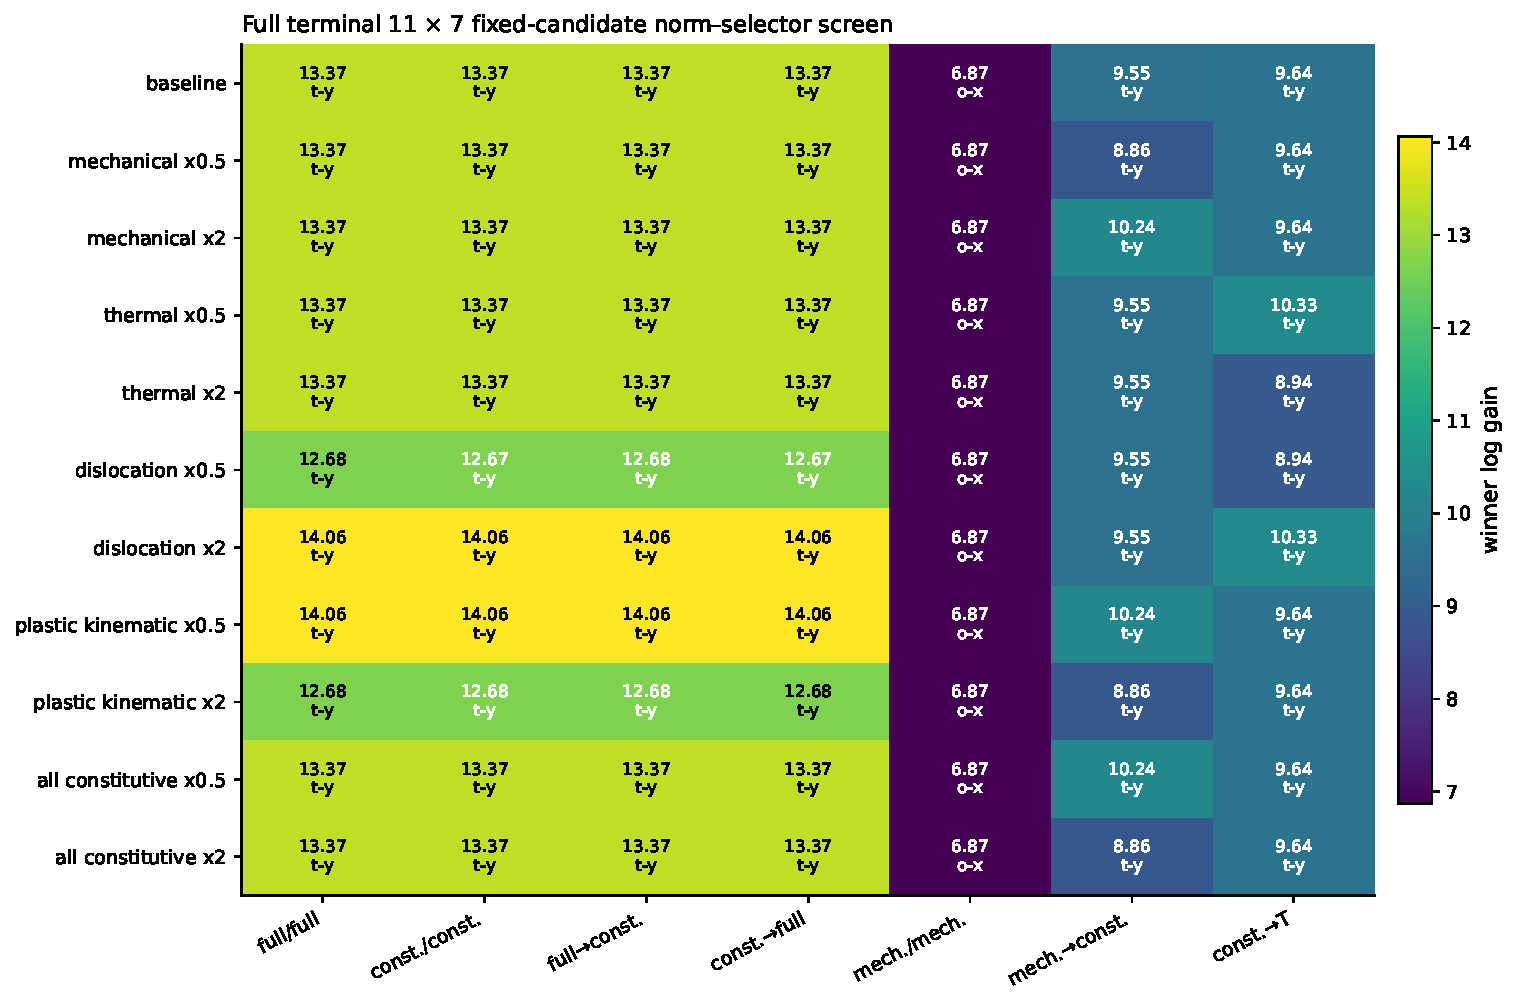
\includegraphics[width=0.92\linewidth]{figS01_full_norm_selector_matrix.pdf}
\caption{Complete terminal fixed-candidate norm--selector matrix. The rows are
the baseline norm and ten factor-two coordinate-scale perturbations; the
columns are all seven declared input--output maps. Cell annotations report
log gain and the winning registered branch.}
\label{fig:s_full_matrix}
\end{figure}
\end{landscape}
\clearpage

\section{Re-optimized direction--wavenumber and matched freezing}
\label{sec:s_reoptimized}

Direction and wavenumber are re-optimized for all seven selectors under the
baseline and four pre-registered adverse norms.  The singular-value audit
applies the formal 5\% relative-gap threshold, and the piecewise-frozen audit
uses exactly the same metric and endpoint selectors as the time-ordered map.
Machine-readable coordinates, gains, complete singular values/vectors,
baseline generators, convergence rows and all optimizer evaluations are
supplied in \path{05_results/ijp_reference_reoptimization_v4.json},
\path{05_results/ijp_reference_reoptimization_v4_arrays.npz} and
\path{05_results/ijp_reference_reoptimization_v4/}.  V3 is retained as the
lower-resolution reconnaissance and as the previous-candidate baseline, not
as the reference optimization result.  The synthesized figure is included in
the main paper rather than duplicated here.

\IfFileExists{tables/ft_reference_reoptimization_v4_table.tex}{%
\begin{landscape}
\begingroup\scriptsize
\setlength{\LTleft}{0pt}\setlength{\LTright}{0pt}\setlength{\tabcolsep}{2pt}
\renewcommand{\arraystretch}{0.95}
\begin{longtable}{@{}p{1.15cm}p{2.55cm}p{3.60cm}rrrrcc@{}}
\caption{Complete direct reference-objective re-optimization.  Every row is refined on the 129-state/four-substep propagator; $\Delta\log G$ is relative to the V3 retained coordinate reevaluated on that same reference map.  Class I is a finite-band interior candidate, LW is a lower-boundary long-wave branch and HF is a high-frequency reversible branch; neither boundary class is interpreted as a localization wavelength.}\label{tab:s_reference_reoptimization}\\
\toprule
Horizon & Norm & Input--output & $k^*$ ($\mathrm{m^{-1}}$) & $\log G$ & $G$ & $\Delta\log G$ & stat.? & class \\
\midrule
\endfirsthead
\toprule
Horizon & Norm & Input--output & $k^*$ ($\mathrm{m^{-1}}$) & $\log G$ & $G$ & $\Delta\log G$ & stat.? & class \\
\midrule
\endhead
onset & all constitutive $\times2$ & constitutive/constitutive & 54550.4 & 0.621942 & 1.86254 & +2.252e-04 & yes & I \\
onset & all constitutive $\times2$ & constitutive$\rightarrow$full & 21315.1 & 2.969294 & 19.4782 & +3.769e-01 & yes & I \\
onset & all constitutive $\times2$ & constitutive$\rightarrow T$ & 300 & 0.000640 & 1.00064 & +6.775e-04 & yes & LW \\
onset & all constitutive $\times2$ & full$\rightarrow$constitutive & 18285.4 & 0.630114 & 1.87782 & +4.711e-03 & yes & I \\
onset & all constitutive $\times2$ & full/full & 283934 & 9.770385 & 17507.5 & +8.736e-02 & yes & HF \\
onset & all constitutive $\times2$ & mechanical$\rightarrow$constitutive & 18358.7 & -1.272480 & 0.280136 & +3.914e-01 & yes & I \\
onset & all constitutive $\times2$ & mechanical/mechanical & 283934 & 9.770385 & 17507.5 & +8.736e-02 & yes & HF \\
onset & baseline & constitutive/constitutive & 54550.4 & 0.621942 & 1.86254 & +2.252e-04 & yes & I \\
onset & baseline & constitutive$\rightarrow$full & 20334.6 & 2.278484 & 9.76187 & +3.977e-01 & yes & I \\
onset & baseline & constitutive$\rightarrow T$ & 300 & 0.000640 & 1.00064 & +6.775e-04 & yes & LW \\
onset & baseline & full$\rightarrow$constitutive & 18322 & 0.655262 & 1.92565 & +1.792e-02 & yes & I \\
onset & baseline & full/full & 283934 & 9.770385 & 17507.5 & +8.736e-02 & yes & HF \\
onset & baseline & mechanical$\rightarrow$constitutive & 18358.7 & -0.579333 & 0.560272 & +3.914e-01 & yes & I \\
onset & baseline & mechanical/mechanical & 283934 & 9.770385 & 17507.5 & +8.736e-02 & yes & HF \\
onset & dislocation $\times2$ & constitutive/constitutive & 80968.6 & 1.093127 & 2.98359 & +2.371e-04 & yes & I \\
onset & dislocation $\times2$ & constitutive$\rightarrow$full & 22306.3 & 2.288688 & 9.86199 & +3.944e-01 & yes & I \\
onset & dislocation $\times2$ & constitutive$\rightarrow T$ & 300 & 0.002454 & 1.00246 & +7.563e-04 & yes & LW \\
onset & dislocation $\times2$ & full$\rightarrow$constitutive & 62926.9 & 1.107570 & 3.02699 & +7.478e-03 & yes & I \\
onset & dislocation $\times2$ & full/full & 283934 & 9.770385 & 17507.5 & +8.736e-02 & yes & HF \\
onset & dislocation $\times2$ & mechanical$\rightarrow$constitutive & 18358.7 & -0.579334 & 0.560271 & +3.914e-01 & yes & I \\
onset & dislocation $\times2$ & mechanical/mechanical & 283934 & 9.770385 & 17507.5 & +8.736e-02 & yes & HF \\
onset & mechanical $\times0.5$ & constitutive/constitutive & 54550.4 & 0.621942 & 1.86254 & +2.252e-04 & yes & I \\
onset & mechanical $\times0.5$ & constitutive$\rightarrow$full & 21315.1 & 2.969294 & 19.4782 & +3.769e-01 & yes & I \\
onset & mechanical $\times0.5$ & constitutive$\rightarrow T$ & 300 & 0.000640 & 1.00064 & +6.775e-04 & yes & LW \\
onset & mechanical $\times0.5$ & full$\rightarrow$constitutive & 18285.4 & 0.630114 & 1.87782 & +4.711e-03 & yes & I \\
onset & mechanical $\times0.5$ & full/full & 283934 & 9.770385 & 17507.5 & +8.736e-02 & yes & HF \\
onset & mechanical $\times0.5$ & mechanical$\rightarrow$constitutive & 18358.7 & -1.272480 & 0.280136 & +3.914e-01 & yes & I \\
onset & mechanical $\times0.5$ & mechanical/mechanical & 283934 & 9.770385 & 17507.5 & +8.736e-02 & yes & HF \\
onset & thermal $\times0.5$ & constitutive/constitutive & 59355.1 & 0.622488 & 1.86356 & +5.519e-04 & yes & I \\
onset & thermal $\times0.5$ & constitutive$\rightarrow$full & 21315.1 & 2.279999 & 9.77667 & +3.993e-01 & yes & I \\
onset & thermal $\times0.5$ & constitutive$\rightarrow T$ & 300 & 0.002455 & 1.00246 & +7.568e-04 & yes & LW \\
onset & thermal $\times0.5$ & full$\rightarrow$constitutive & 18322 & 0.655886 & 1.92685 & +1.793e-02 & yes & I \\
onset & thermal $\times0.5$ & full/full & 283934 & 9.770385 & 17507.5 & +8.736e-02 & yes & HF \\
onset & thermal $\times0.5$ & mechanical$\rightarrow$constitutive & 18358.7 & -0.578156 & 0.560932 & +3.914e-01 & yes & I \\
onset & thermal $\times0.5$ & mechanical/mechanical & 283934 & 9.770385 & 17507.5 & +8.736e-02 & yes & HF \\
terminal & all constitutive $\times2$ & constitutive/constitutive & 7724.01 & 13.367382 & 638823 & +5.197e-03 & yes & I \\
terminal & all constitutive $\times2$ & constitutive$\rightarrow$full & 7724.01 & 13.368115 & 639291 & +0.000e+00 & yes & I \\
terminal & all constitutive $\times2$ & constitutive$\rightarrow T$ & 7724.01 & 9.636463 & 15313.1 & +0.000e+00 & yes & I \\
terminal & all constitutive $\times2$ & full$\rightarrow$constitutive & 7724.01 & 13.367443 & 638861 & +5.347e-03 & yes & I \\
terminal & all constitutive $\times2$ & full/full & 7724.01 & 13.368175 & 639329 & +0.000e+00 & yes & I \\
terminal & all constitutive $\times2$ & mechanical$\rightarrow$constitutive & 6592.74 & 9.181419 & 9714.93 & +8.916e-01 & yes & I \\
terminal & all constitutive $\times2$ & mechanical/mechanical & 300000 & 9.583252 & 14519.6 & +0.000e+00 & yes & HF \\
terminal & baseline & constitutive/constitutive & 7724.01 & 13.367382 & 638823 & +5.197e-03 & yes & I \\
terminal & baseline & constitutive$\rightarrow$full & 7724.01 & 13.367566 & 638940 & +5.168e-03 & yes & I \\
terminal & baseline & constitutive$\rightarrow T$ & 7724.01 & 9.636463 & 15313.1 & +0.000e+00 & yes & I \\
terminal & baseline & full$\rightarrow$constitutive & 7724.01 & 13.367623 & 638977 & +5.830e-03 & yes & I \\
terminal & baseline & full/full & 7724.01 & 13.367806 & 639094 & +0.000e+00 & yes & I \\
terminal & baseline & mechanical$\rightarrow$constitutive & 6592.74 & 9.874566 & 19429.9 & +8.916e-01 & yes & I \\
terminal & baseline & mechanical/mechanical & 300000 & 9.583252 & 14519.6 & +0.000e+00 & yes & HF \\
terminal & dislocation $\times2$ & constitutive/constitutive & 7724.01 & 14.060494 & 1.2776e+06 & +5.315e-03 & yes & I \\
terminal & dislocation $\times2$ & constitutive$\rightarrow$full & 7724.01 & 14.060677 & 1.27783e+06 & +5.167e-03 & yes & I \\
terminal & dislocation $\times2$ & constitutive$\rightarrow T$ & 7724.01 & 10.329573 & 30625 & +0.000e+00 & yes & I \\
terminal & dislocation $\times2$ & full$\rightarrow$constitutive & 7724.01 & 14.060554 & 1.27768e+06 & +5.428e-03 & yes & I \\
terminal & dislocation $\times2$ & full/full & 7724.01 & 14.060737 & 1.27791e+06 & +0.000e+00 & yes & I \\
terminal & dislocation $\times2$ & mechanical$\rightarrow$constitutive & 6592.74 & 9.874566 & 19429.9 & +8.916e-01 & yes & I \\
terminal & dislocation $\times2$ & mechanical/mechanical & 300000 & 9.583252 & 14519.6 & +0.000e+00 & yes & HF \\
terminal & mechanical $\times0.5$ & constitutive/constitutive & 7724.01 & 13.367382 & 638823 & +5.197e-03 & yes & I \\
terminal & mechanical $\times0.5$ & constitutive$\rightarrow$full & 7724.01 & 13.368115 & 639291 & +0.000e+00 & yes & I \\
terminal & mechanical $\times0.5$ & constitutive$\rightarrow T$ & 7724.01 & 9.636463 & 15313.1 & +0.000e+00 & yes & I \\
terminal & mechanical $\times0.5$ & full$\rightarrow$constitutive & 7724.01 & 13.367443 & 638861 & +5.347e-03 & yes & I \\
terminal & mechanical $\times0.5$ & full/full & 7724.01 & 13.368175 & 639329 & +0.000e+00 & yes & I \\
terminal & mechanical $\times0.5$ & mechanical$\rightarrow$constitutive & 6592.74 & 9.181419 & 9714.93 & +8.916e-01 & yes & I \\
terminal & mechanical $\times0.5$ & mechanical/mechanical & 300000 & 9.583252 & 14519.6 & +0.000e+00 & yes & HF \\
terminal & thermal $\times0.5$ & constitutive/constitutive & 7724.01 & 13.368209 & 639351 & +5.246e-03 & yes & I \\
terminal & thermal $\times0.5$ & constitutive$\rightarrow$full & 7724.01 & 13.368392 & 639468 & +5.149e-03 & yes & I \\
terminal & thermal $\times0.5$ & constitutive$\rightarrow T$ & 7724.01 & 10.329575 & 30625.1 & +0.000e+00 & yes & I \\
terminal & thermal $\times0.5$ & full$\rightarrow$constitutive & 7724.01 & 13.368450 & 639505 & +5.848e-03 & yes & I \\
terminal & thermal $\times0.5$ & full/full & 7724.01 & 13.368633 & 639622 & +0.000e+00 & yes & I \\
terminal & thermal $\times0.5$ & mechanical$\rightarrow$constitutive & 6592.74 & 9.875435 & 19446.8 & +8.916e-01 & yes & I \\
terminal & thermal $\times0.5$ & mechanical/mechanical & 300000 & 9.583252 & 14519.6 & +0.000e+00 & yes & HF \\
\bottomrule
\end{longtable}
\endgroup
\end{landscape}

\begin{table}[ht]
\centering
\caption{Sampled near-optimal sets for the baseline constitutive/constitutive map.  The audit combines an independent scrambled-Sobol challenge with local direction rings and full-domain fixed-direction wavenumber profiles; it is not a continuum global certificate.}
\begin{tabular}{@{}lrrrr@{}}
\toprule
Horizon/$\varepsilon$ & members & $k_{\min}$ ($\mathrm{m^{-1}}$) & $k_{\max}$ ($\mathrm{m^{-1}}$) & max angle (deg) \\
\midrule
onset/0.1\% & 414 & 1194.32 & 300000 & 89.451 \\
onset/0.5\% & 713 & 346.12 & 300000 & 89.951 \\
onset/1.0\% & 760 & 300 & 300000 & 89.951 \\
onset/2.0\% & 760 & 300 & 300000 & 89.951 \\
terminal/0.1\% & 3 & 7535.66 & 7724.01 & 0.012 \\
terminal/0.5\% & 5 & 7535.66 & 8455.15 & 0.012 \\
terminal/1.0\% & 8 & 6716.16 & 8455.15 & 0.012 \\
terminal/2.0\% & 10 & 6716.16 & 9486.83 & 0.012 \\
\bottomrule
\end{tabular}
\end{table}
%
}{\emph{The direct reference-objective table is generated by
\path{tools/build_ijp_v4_supplement_tables.py}.}}

\section{Loading transfer, local sensitivity and titanium landmarks}

The V3 table directory supplies the three added loading cases, the
branch-local $\pm20\%$ sensitivity records and logarithmic derivatives, and
the bounded external check against synchronized Grade-II CP-Ti
stress/temperature landmarks.  The latter is a timing-and-scale check, not a
batch-calibrated validation.  The figure synthesized from those tables is
included in the main paper.

\section{Full-grid convergence, branch switching and physical metrics}

The V4 full-grid receipt
\path{05_results/ijp_v4_full_fourier_convergence_audit_v1.json} supplies the
raw Nyquist negative control, matched no-Nyquist control, two-thirds-dealiased
16/32/64-cell ladder, independent time-step and integration-format checks,
and the first-failure equation--variable--wavenumber record.  The separate
receipt \path{05_results/ijp_v4_start_branch_metric_audit_v1.json} supplies
the initial-time sensitivity, all detected branch transitions, four bounded
propagation conventions, and the positive-energy-subspace metric audit.  The
resolved gain converges, while the discarded nonlinear right-hand-side energy
keeps complete harmonic closure open.

\begin{table}[ht]
\centering
\caption{Registered active-set events on the factor-64 base history.  The
category signs give the one-sided branch labels; event times are secant
estimates inside the listed checkpoint intervals.}
\small
\begin{tabular}{@{}llll@{}}
\toprule
Event time ($\mu$s) & Changed contracts & Category change & Role \\
\midrule
0.765638 & slip04 yield/rate sign & $0\rightarrow-1$ & activation \\
0.775926 & slip06 yield/rate sign & $0\rightarrow-1$ & activation \\
1.601157 & slip07/slip13 yield/rate sign & $0\rightarrow(+1,-1)$ & activation \\
2.016486 & slip07/slip13 yield/rate sign & $(+1,-1)\rightarrow0$ & deactivation \\
\bottomrule
\end{tabular}
\end{table}

The minimum absolute secant event rate is
$1.72\times10^{13}~\mathrm{Pa\,s^{-1}}$ and the maximum thermally activated
threshold-rate jump is $1.97\times10^{-13}~\mathrm{s^{-1}}$, or
$1.97\times10^{-17}$ of the imposed shear rate.  The corresponding maximum
left/right/secant convention change in terminal gain is 0.0622\%.

\begin{table}[ht]
\centering
\caption{Positive-energy-subspace and nullspace-invariance audit.  Relative
leakage above $10^{-10}$ rejects a quotient-space interpretation.}
\begin{tabular}{@{}lrrrrr@{}}
\toprule
Horizon & rank/nullity & $G_{E\rightarrow E}$ & $G_{E\rightarrow O}$ & $E\rightarrow E$ leakage & quotient? \\
\midrule
Near onset & 28/41 & 1.002 & 1.697 & $2.38\times10^{-4}$ & no \\
Terminal & 28/41 & 117.37 & 73.16 & 0.9996 & no \\
\bottomrule
\end{tabular}
\end{table}

\section{Reproducibility contracts}

The complete direct-reference receipt is
\path{05_results/ijp_reference_reoptimization_v4.json}; the V3 reconnaissance
receipt is retained at \path{05_results/ijp_revision_evidence_v3.json}.  The exact literature
landmarks and extraction record are under
\path{04_reproducibility/literature_digitization/guo2019_prl/}.  Parameter
source keys S2--S5 identify the exact reference record or paper, frozen kernel
version, public repository commit, configuration paths, SHA-256 checksums and
access date.

\end{document}
